\documentclass{article}


\usepackage{arxiv}

\usepackage{placeins}
\usepackage[utf8]{inputenc} % allow utf-8 input
\usepackage[T1]{fontenc}    % use 8-bit T1 fonts
\usepackage{hyperref}       % hyperlinks
\usepackage{url}            % simple URL typesetting
\usepackage{booktabs}       % professional-quality tables
\usepackage{amsfonts}       % blackboard math symbols
\usepackage{nicefrac}       % compact symbols for 1/2, etc.
\usepackage{microtype}      % microtypography

\usepackage{graphicx}	% to insert graphs
\usepackage{caption}	% to customize caption style
\usepackage{float}
\usepackage{subfigure}

\usepackage{amsmath}

\title{COMP0037 ASSIGNMENT 2}


\author{
 Group: \texttt{Group L}\\
}

%\date{}

\begin{document}

\maketitle

\captionsetup[figure]{labelformat={default},labelsep=period,name={Fig.}}

% -------------------------------------------------------------------------------------------
\section{Reactive Planner}
% -----------
\subsection {Reactive Planning System}

A reactive planning system works like that: The planner makes a trajectory using the latest world model and the free space assumption. And the robot constantly perceives the environment and updates the world map as it moves. When the original path has become blocked by an obstacle, it reacts by planning a new set of actions and plans. See the block diagram in Fig. \ref {fig:reactivePlanningSystem}.

\begin{figure}[ht]
\centering
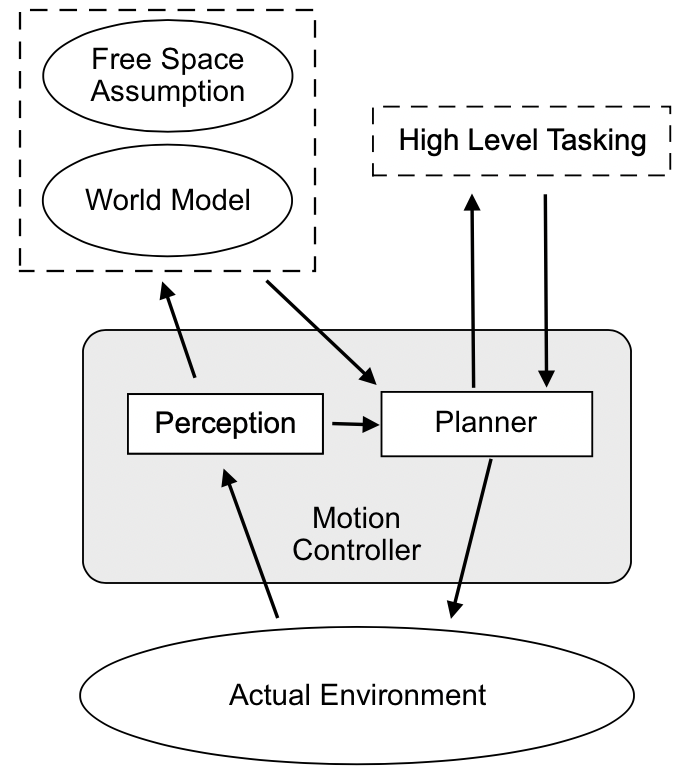
\includegraphics[scale=0.5]{graphs/part1/reactivePlanningSystem.PNG}
\caption{Reactive Planning System}
\label{fig:reactivePlanningSystem}
\end{figure}

% -----------
\subsection {Our Implementation}

We implement the reactive planning system by complete the function \textit{checkIfCurrentPathIsStillGood} in the \textit{ReactivePlannerContoller.py}. The code is shown in Fig. \ref{fig:code}.

\begin{figure}[ht]
\centering
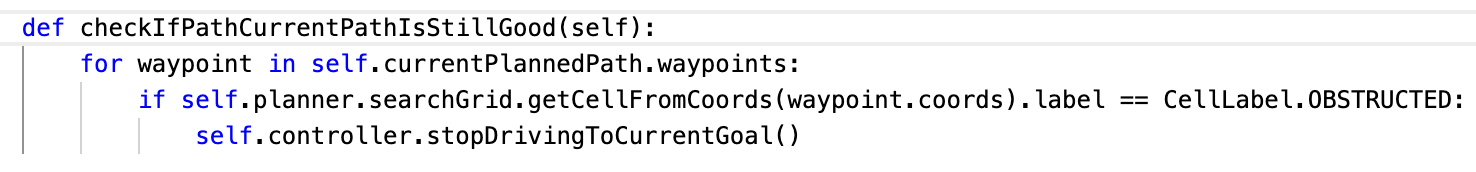
\includegraphics[scale=0.6]{graphs/part1/code.PNG}
\caption{}
\label{fig:code}
\end{figure}

The result is shown in Fig.\ref{fig:result1} and Fig.\ref{fig:result2}.

\begin{figure}[H]
\centering  
\subfigure[STDR GUI]{
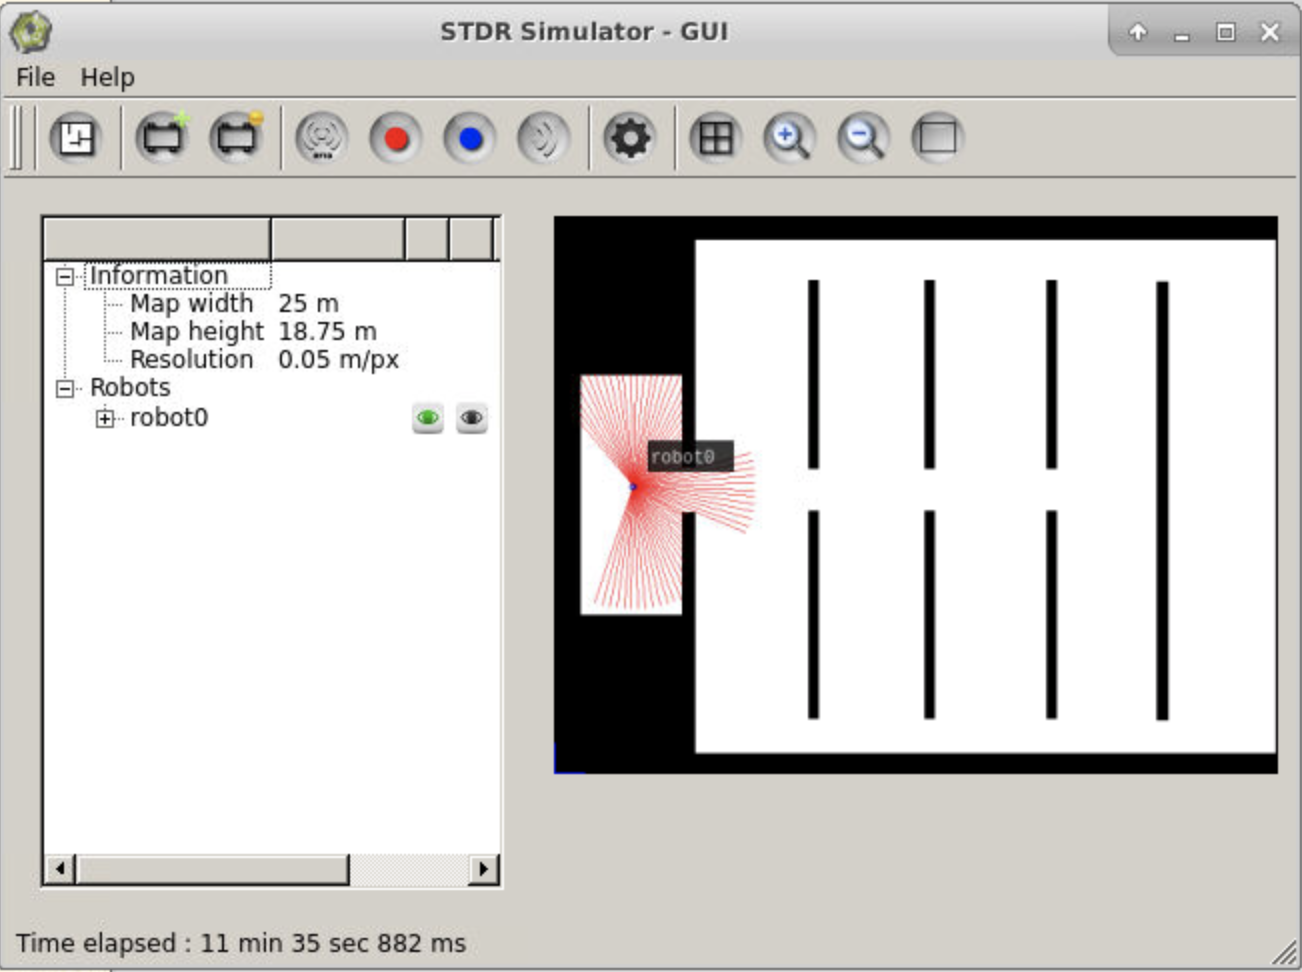
\includegraphics[width=0.45\textwidth]{graphs/part1/1-1/GUI.png}}
\subfigure[Planner Occupancy Grid]{
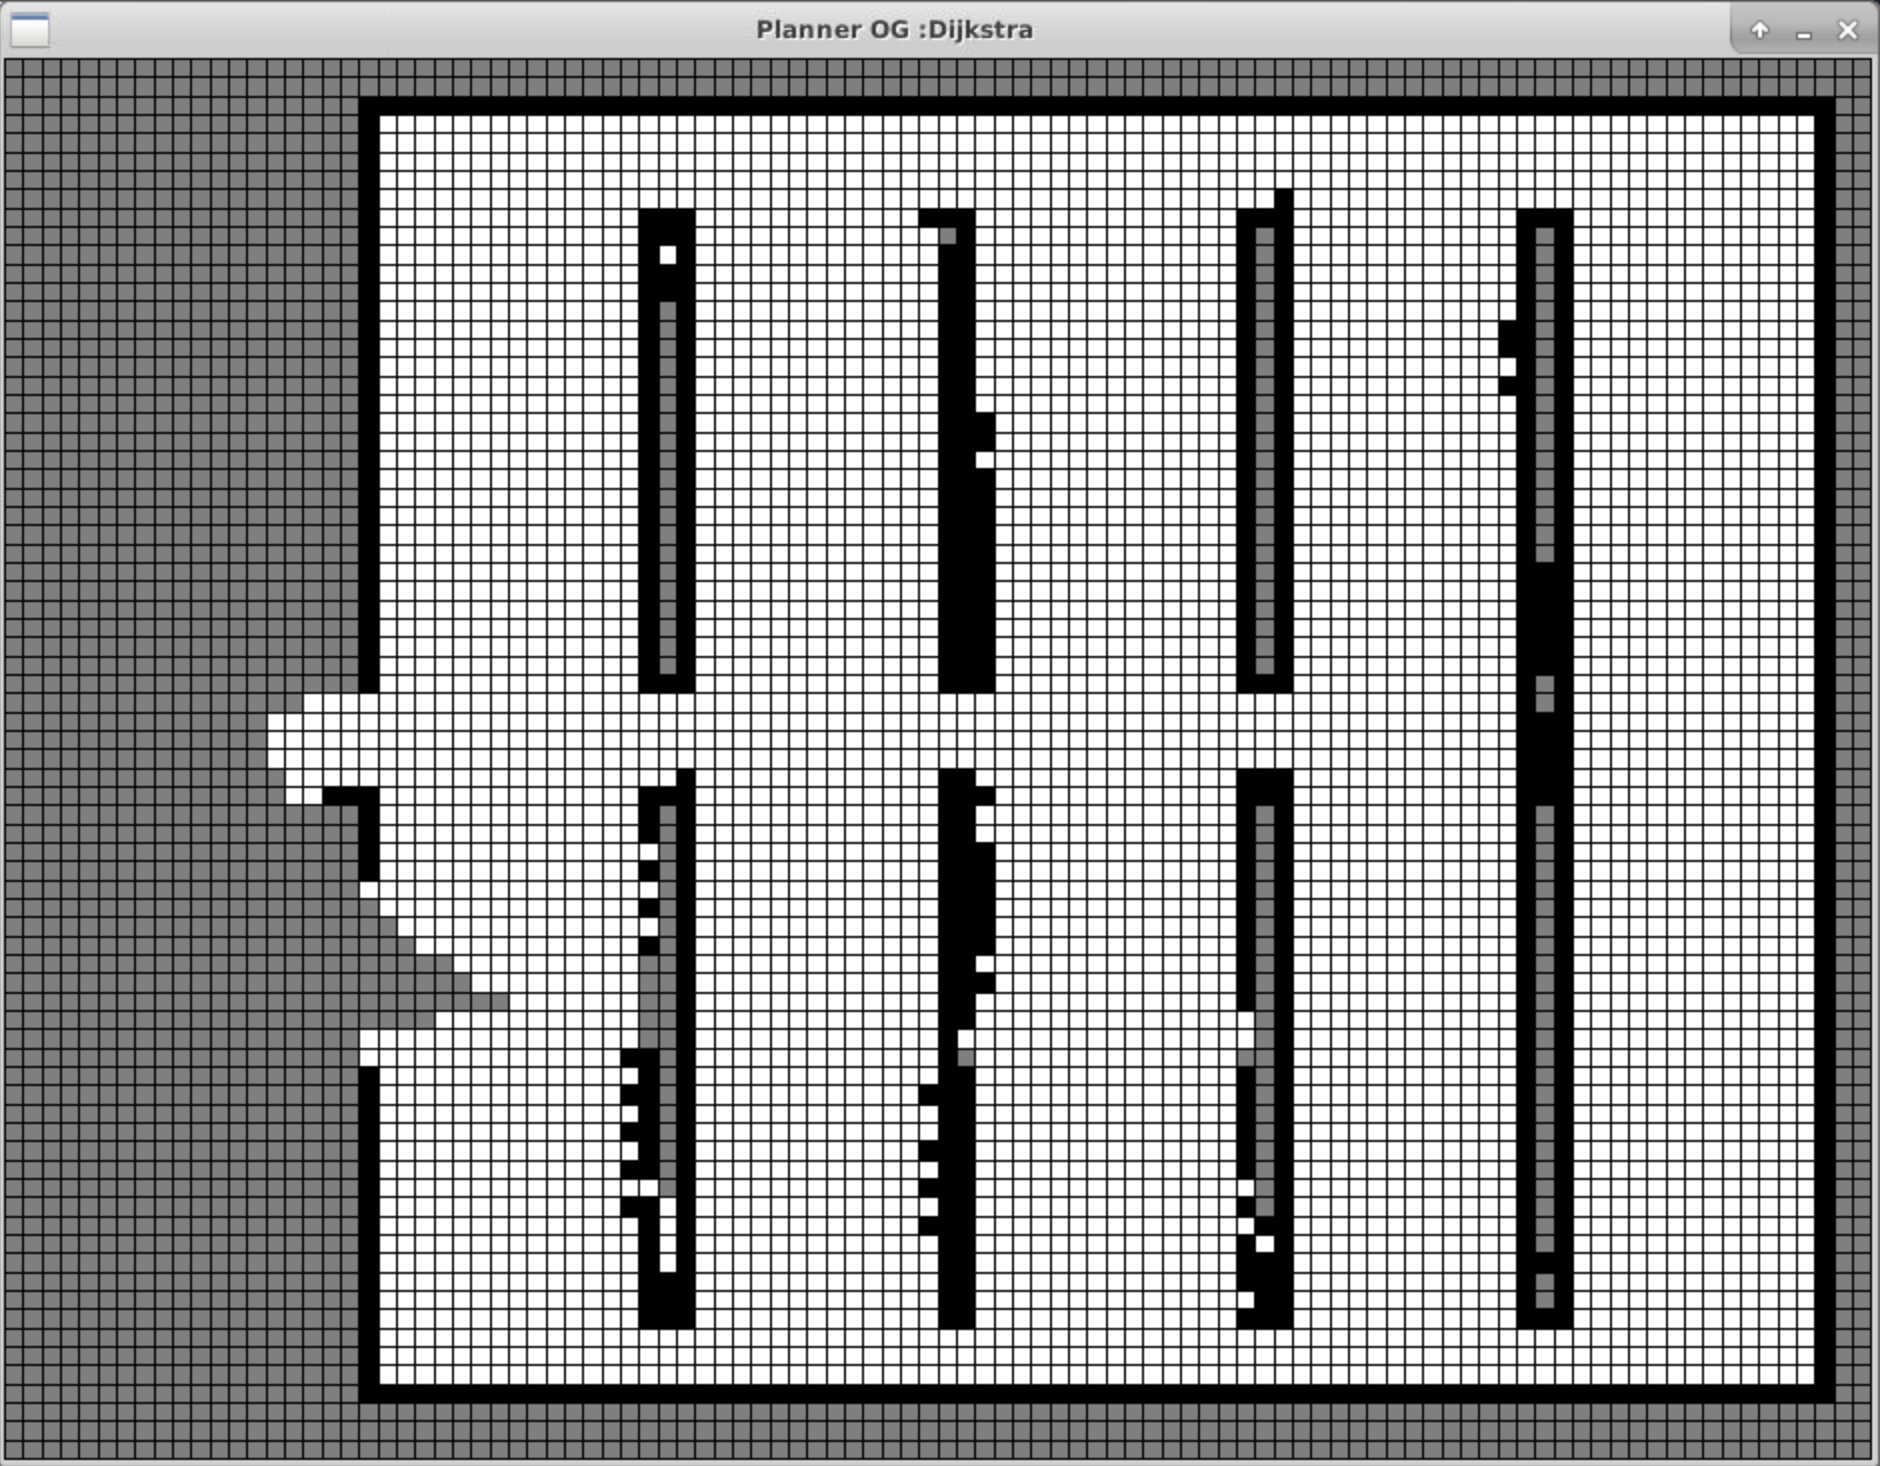
\includegraphics[width=0.45\textwidth]{graphs/part1/1-1/plannerOG.png}}
\subfigure[Planner Search Grid]{
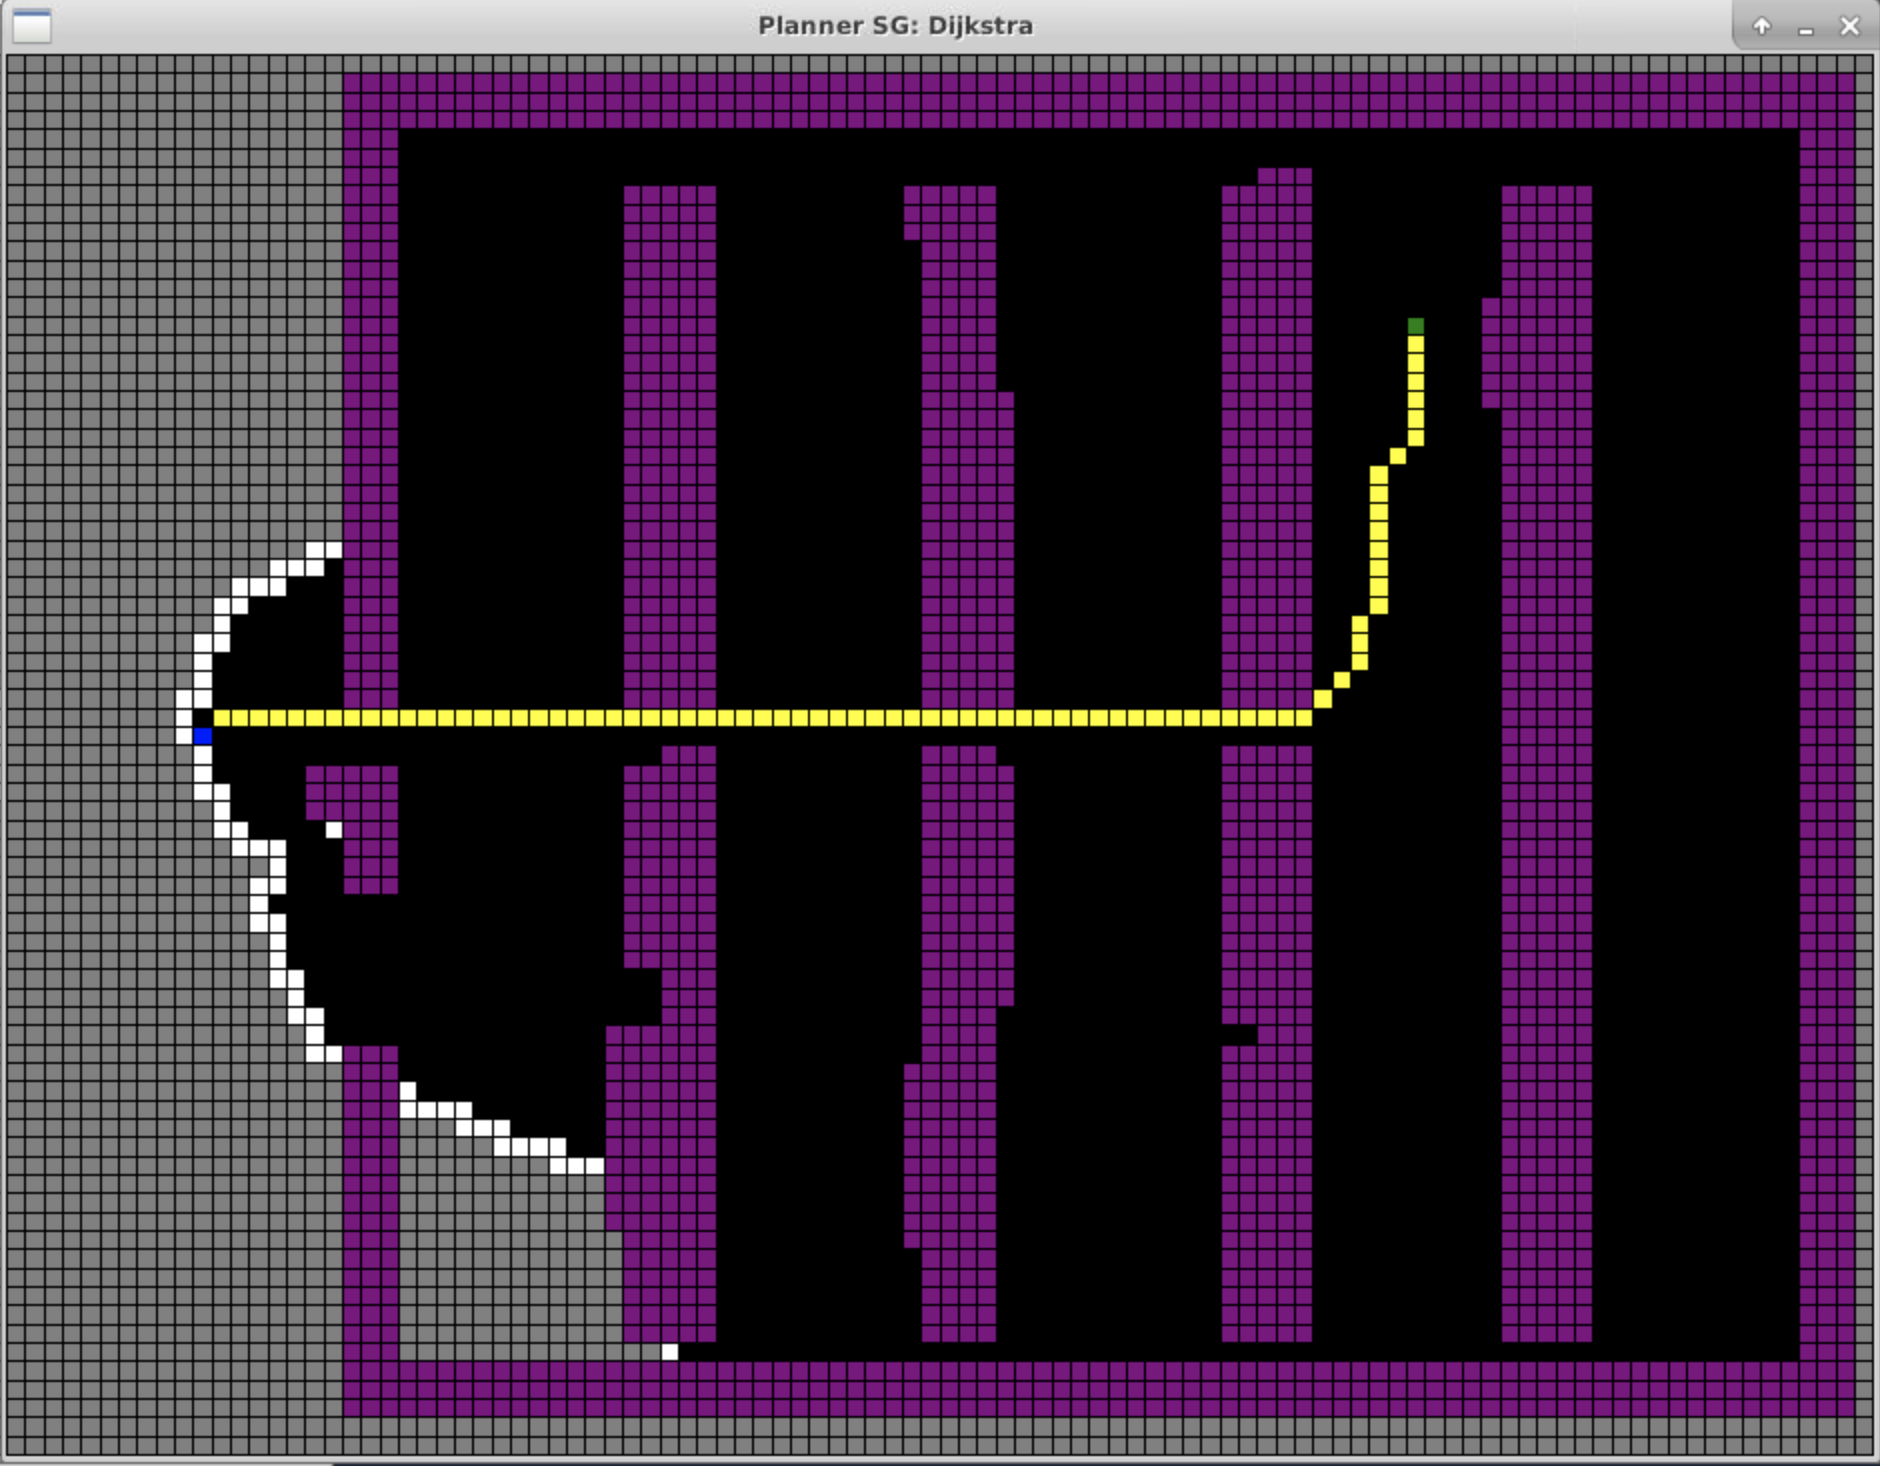
\includegraphics[width=0.45\textwidth]{graphs/part1/1-1/plannerSG.png}}
\subfigure[Mapper Node Occupancy Grid]{
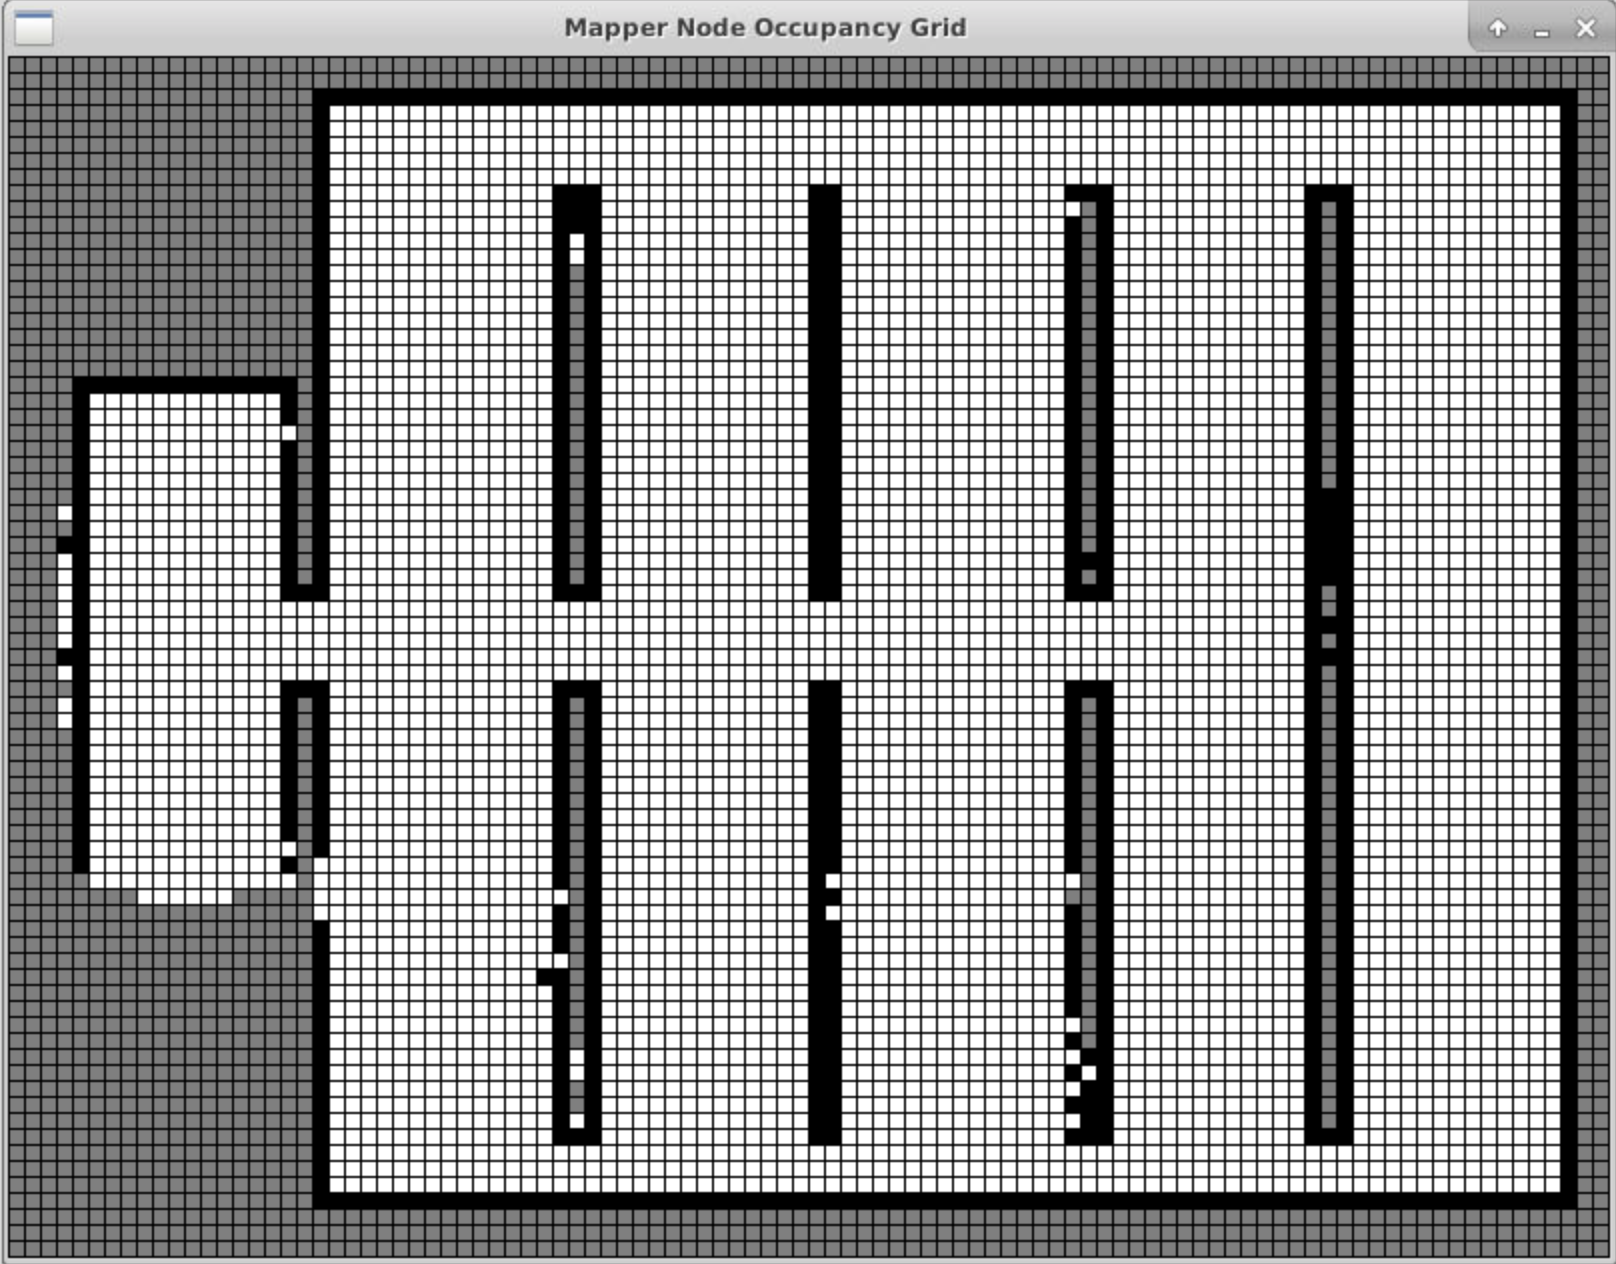
\includegraphics[width=0.45\textwidth]{graphs/part1/1-1/mapperNodeOG.png}}
\caption{Result on the first launch script}
\label{fig:result1}
\end{figure}

\begin{figure}[H]
\centering  
\subfigure[STDR GUI]{
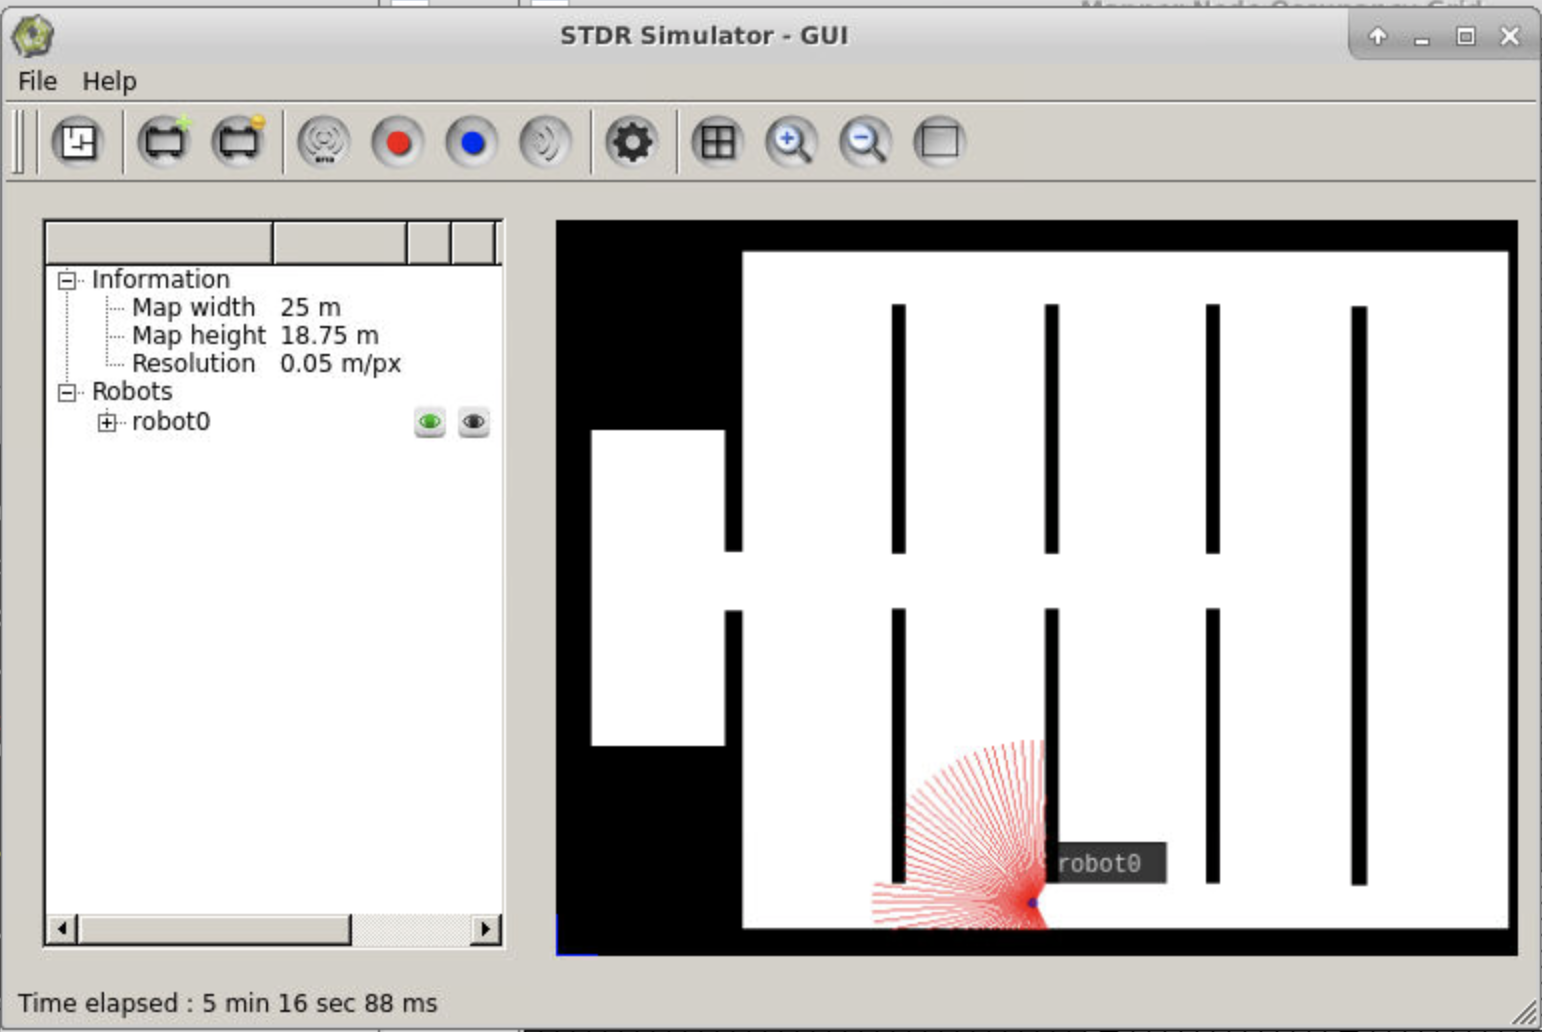
\includegraphics[width=0.45\textwidth]{graphs/part1/1-2/GUI.png}}
\subfigure[Planner Occupancy Grid]{
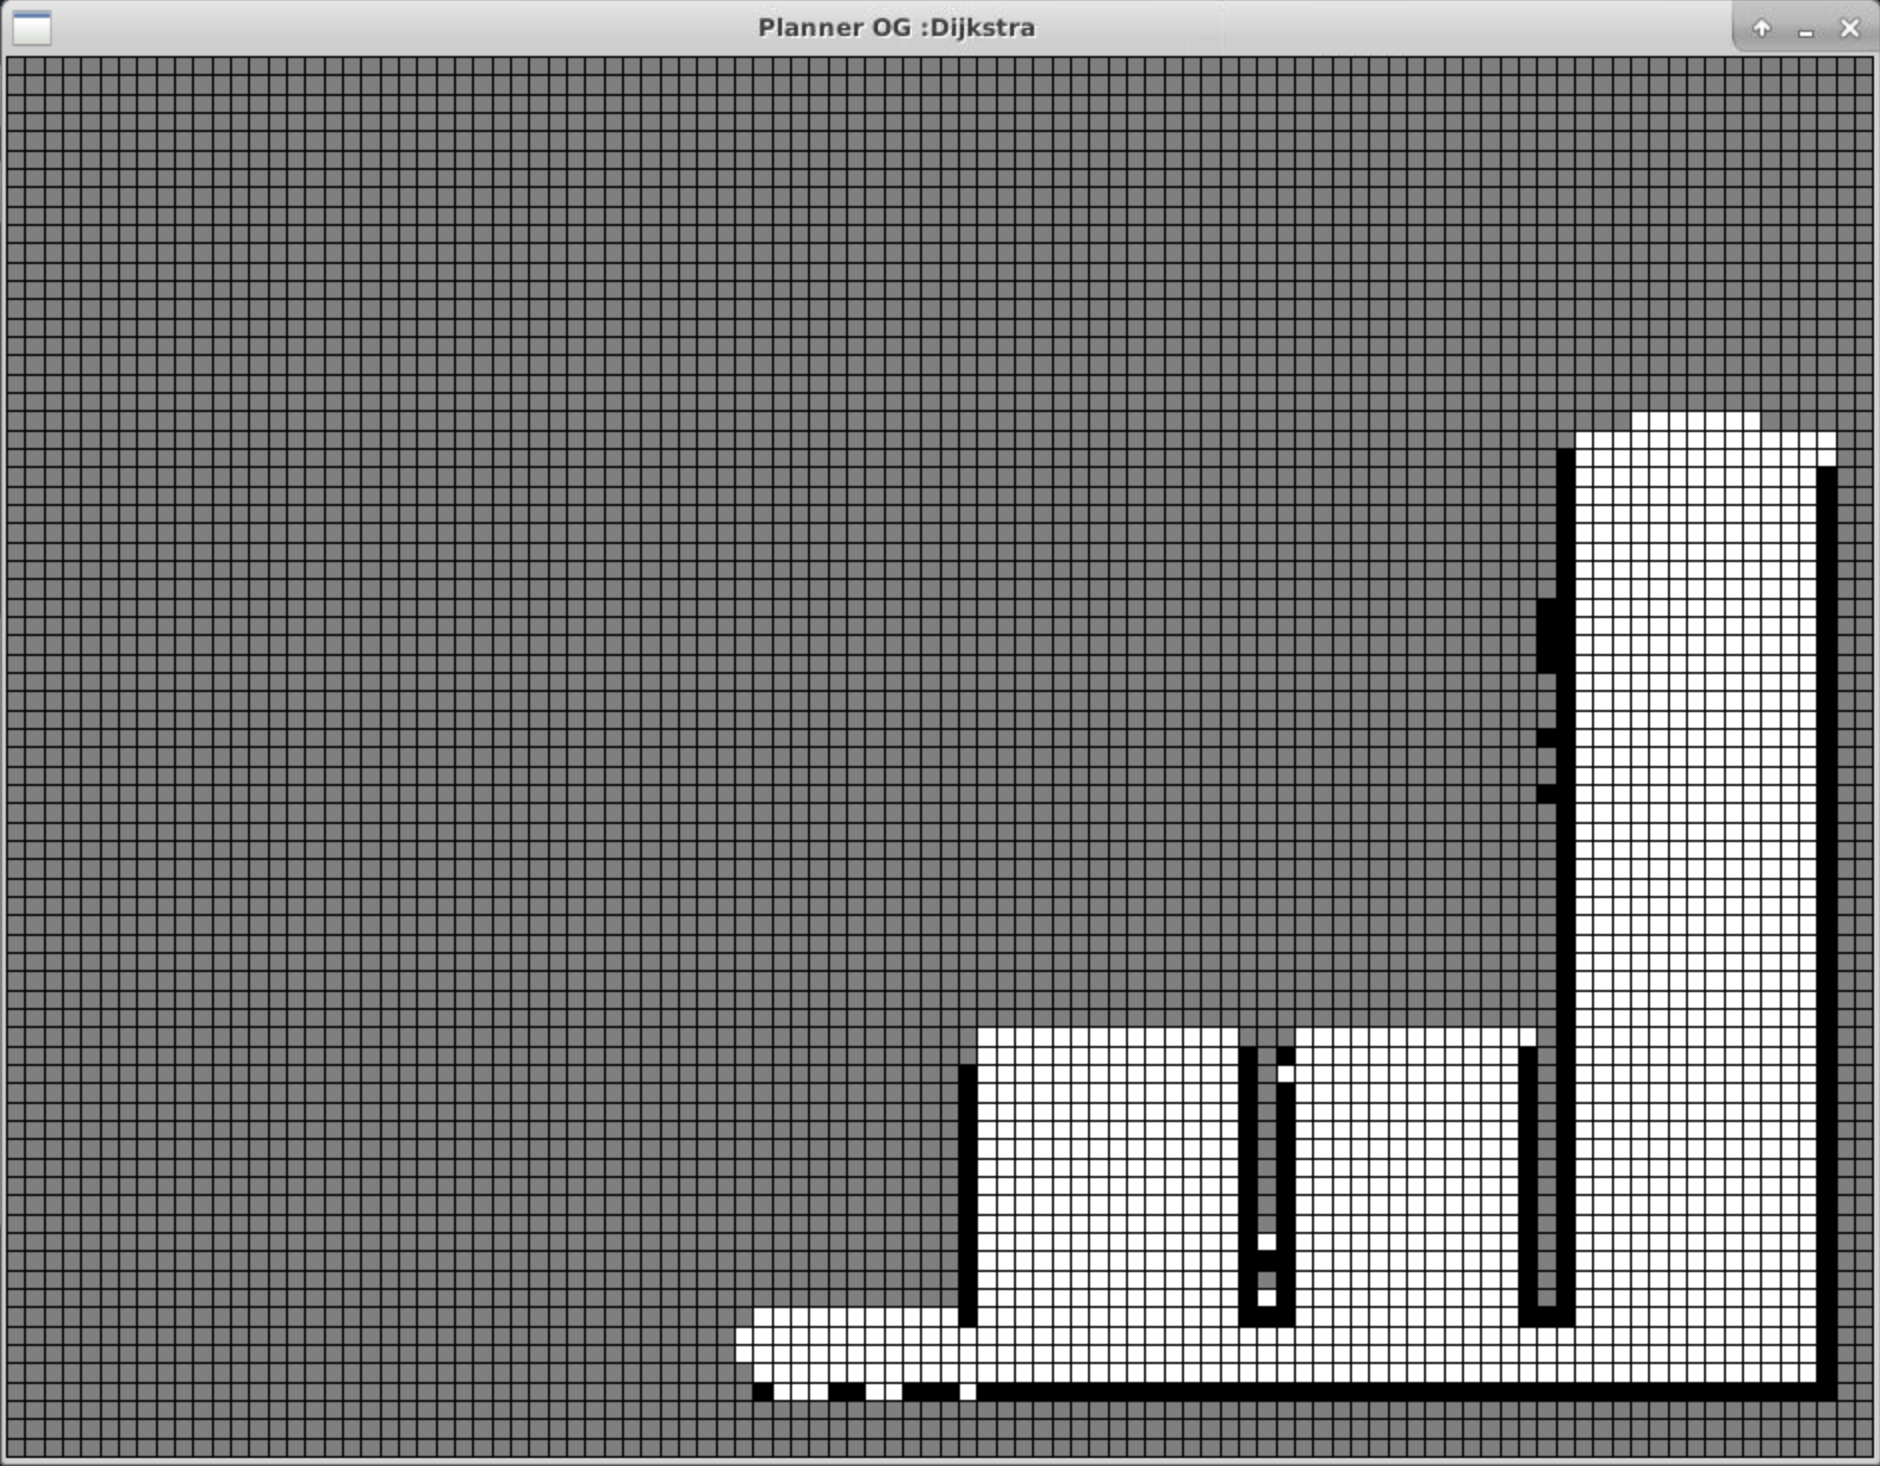
\includegraphics[width=0.45\textwidth]{graphs/part1/1-2/plannerOG.png}}
\subfigure[Planner Search Grid]{
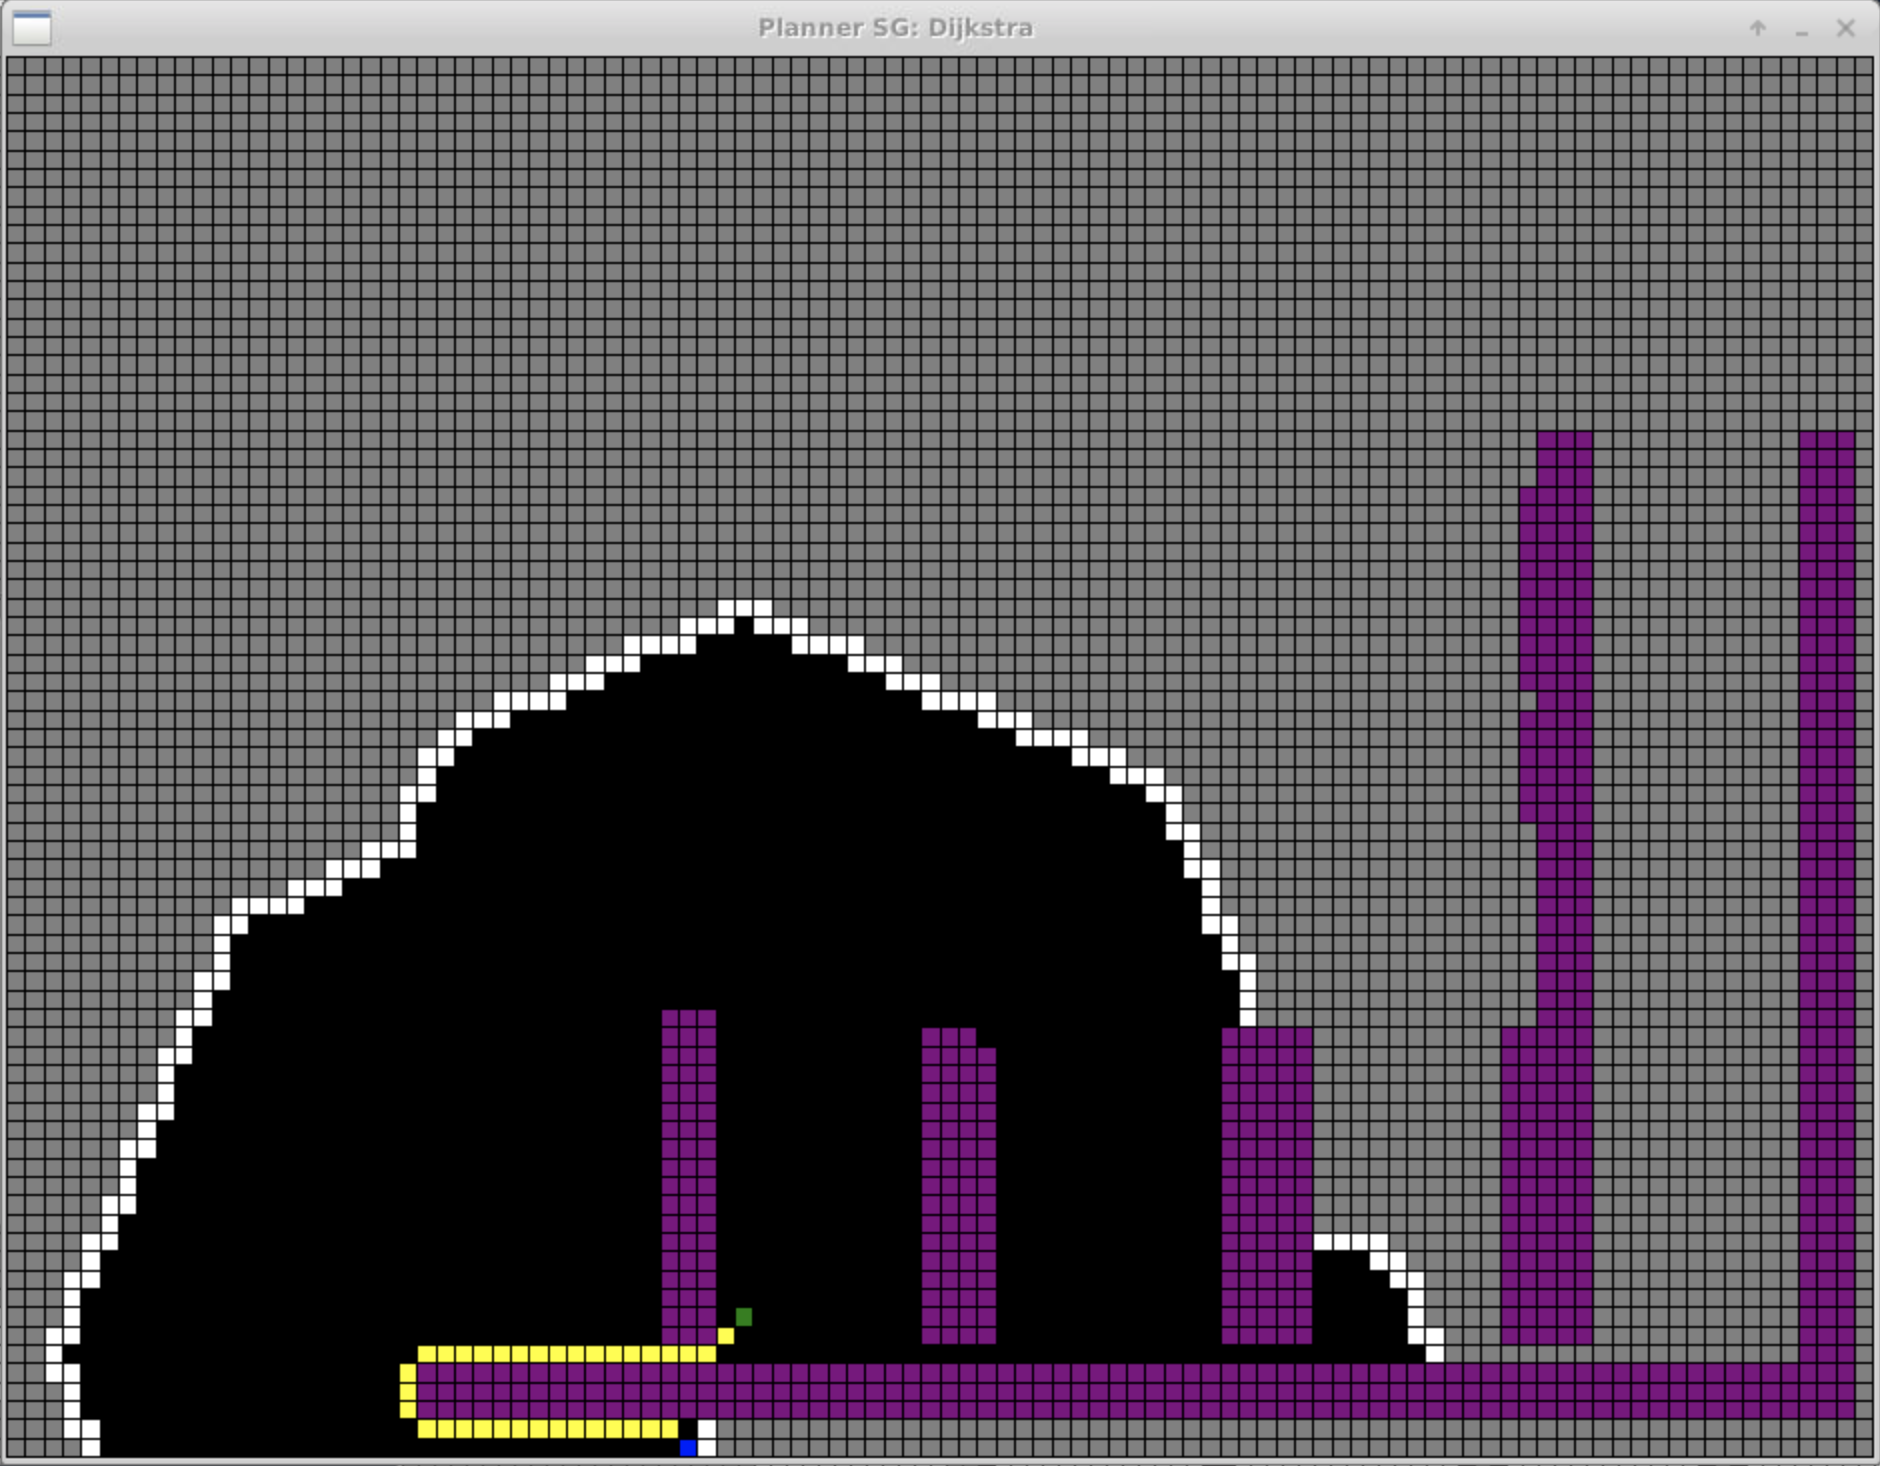
\includegraphics[width=0.45\textwidth]{graphs/part1/1-2/plannerSG.png}}
\subfigure[Mapper Node Occupancy Grid]{
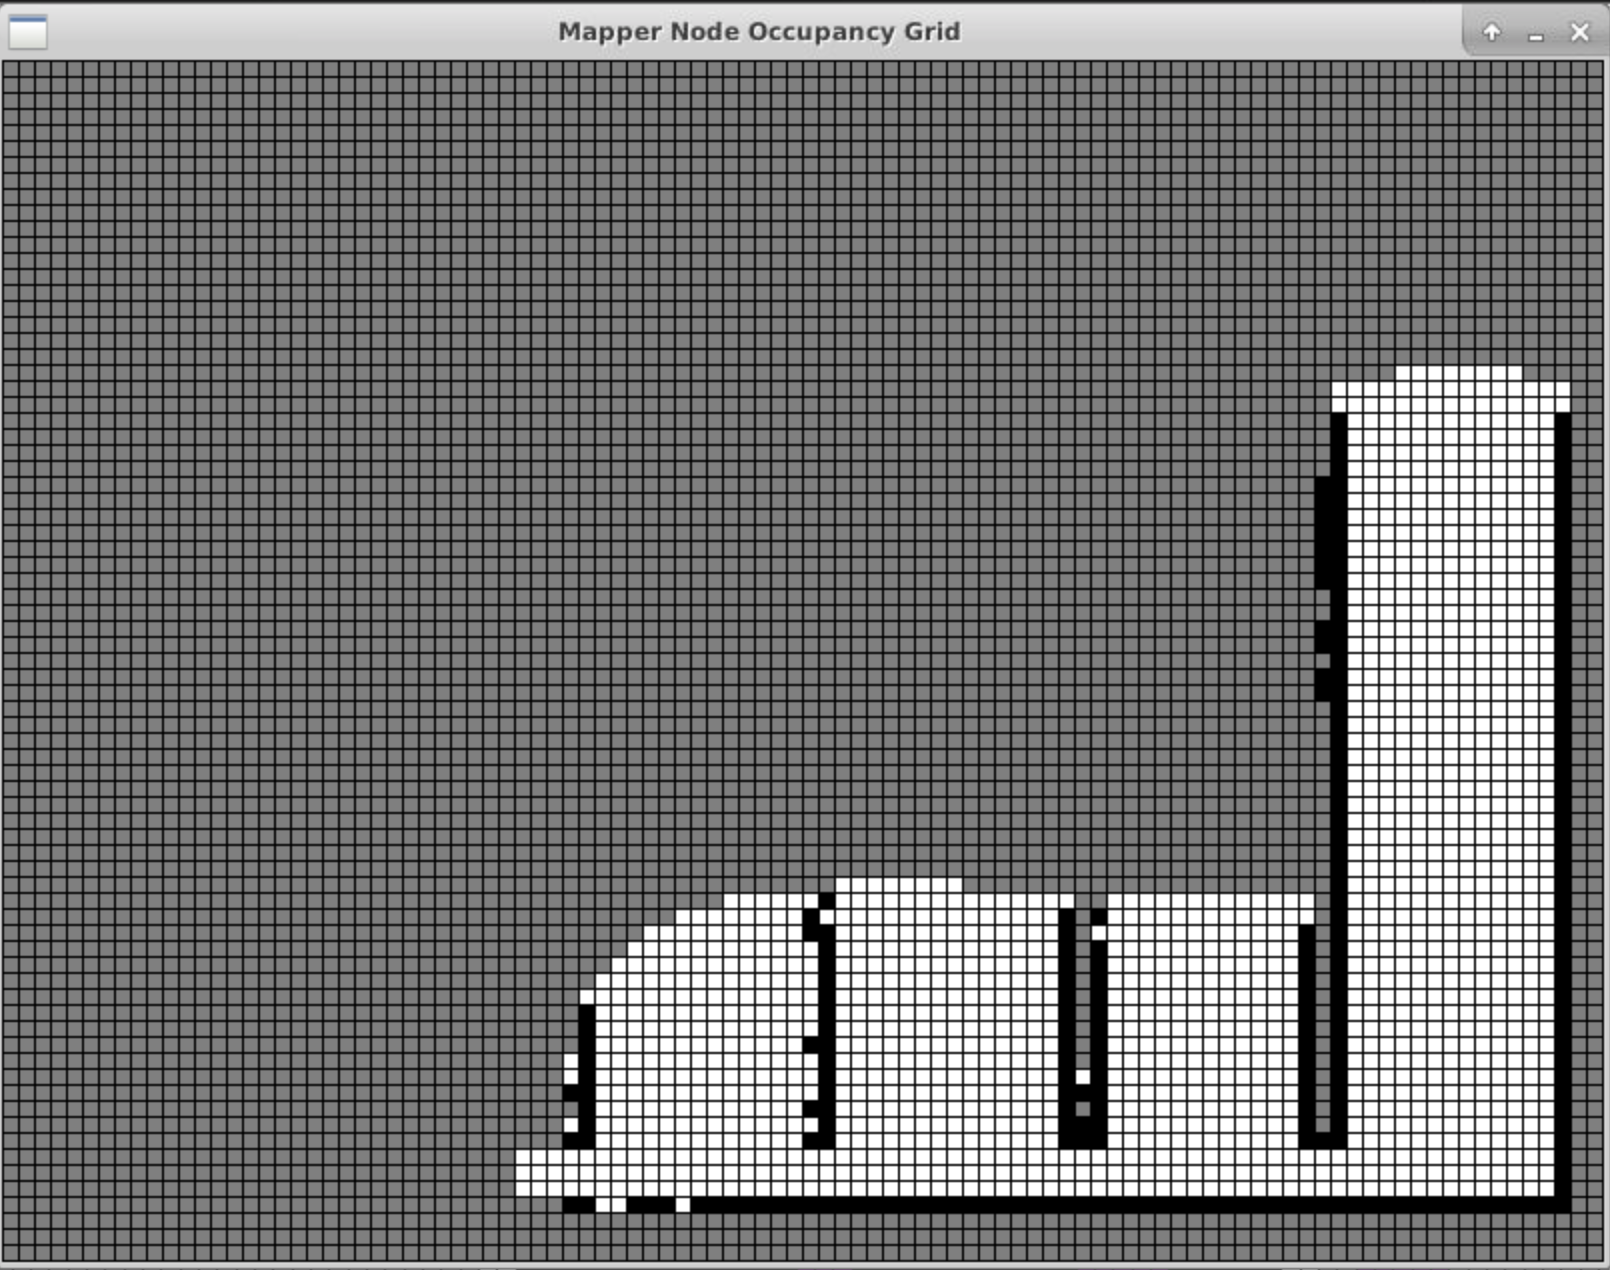
\includegraphics[width=0.45\textwidth]{graphs/part1/1-2/mapperNodeOG.png}}
\caption{Result on the second launch script}
\label{fig:result2}
\end{figure}

% -----------
\subsection {Approach for Improving the Performance}

One approach for improving the performance is using a more efficient global planner to reduce the computational cost associated with re-planning. D*-Lite is one such algorithm that caches previous searches and update them only when we need to. It make use of the backwards search. The graph additionally contains a consistency condition. When the graph changes, such as due to an obstacle, the consistency condition is violated. A priority queue is then used to sort the effect of the failed condition on the path. The highest priority updates are committed first.

\pagebreak
% -------------------------------------------------------------------------------------------
\section{Frontier-Based Exploration System}
% ----------------
\subsection {Frontiers}

A frontier is a cell which its state is known while it is adjacent to a cell whose state is not known. Frontier cells define boundary between open space and the uncharted territory. In frontier-based exploration, the robot moves to the boundary to gain the newest information about the world.

Two methods for identifying frontiers are wave front detection and fast frontier detection.The wave front detection explores the map based on the map that has already been explored. It searches the frontiers using depth-first search, starting from the robot initial location. Once a cell is encountered that looks like a frontier, it pauses the search and traces along all the frontier cells. The latter relies on the newly collected sensor information. The sensor data is used to create a contour, which then be separated into frontier and non-frontier segments. The frontier segments are managed in a database to make them persistent. When data becomes available, the frontiers will be split or merged deleted. One heuristic for choosing next waypoint is picking the closest frontier to the robot. Another one is picking the largest frontier cell.

% ----------------
\subsection {The Exploration Algorithm Provided}
The method provided finds frontiers by traverse all the cells on the occupancy grid each time. Once a frontier is found, it checks if it is in the blacklist. If not, it then calculates the distance between the cell and the centre of the leftmost boundary and see if its distance is smaller than the current smallest value.  Finally, the frontier with the smallest distance (to the centre of the left boundary of the grid) is chose to be the next destination.  

This method is extremely slow since the standard cell to compare the distance is the centre of the left boundary and also there are three nested loops to be run for each time the function is called. Especially the former, setting the standard cell to the midpoint makes the robot shift around the horizontal symmetry axis line by line, which significantly increases distance it needs to travel between two destinations and thus the time used to explore the map. The total time used and the map coverage is averagely around 1500 seconds (25 minutes) and 78\%. 

% ----------------
\subsection {Our Implementation}
We chose the wave front detection algorithm to implement. For choosing the next point, it will pick the cell with the smallest distance from the search start cell, which is the current robot position. (See the key code in Fig. \ref{fig:waveFrontDetection} and Fig. \ref{fig:closestHeuristic}). 

\begin{figure}[ht]
\centering
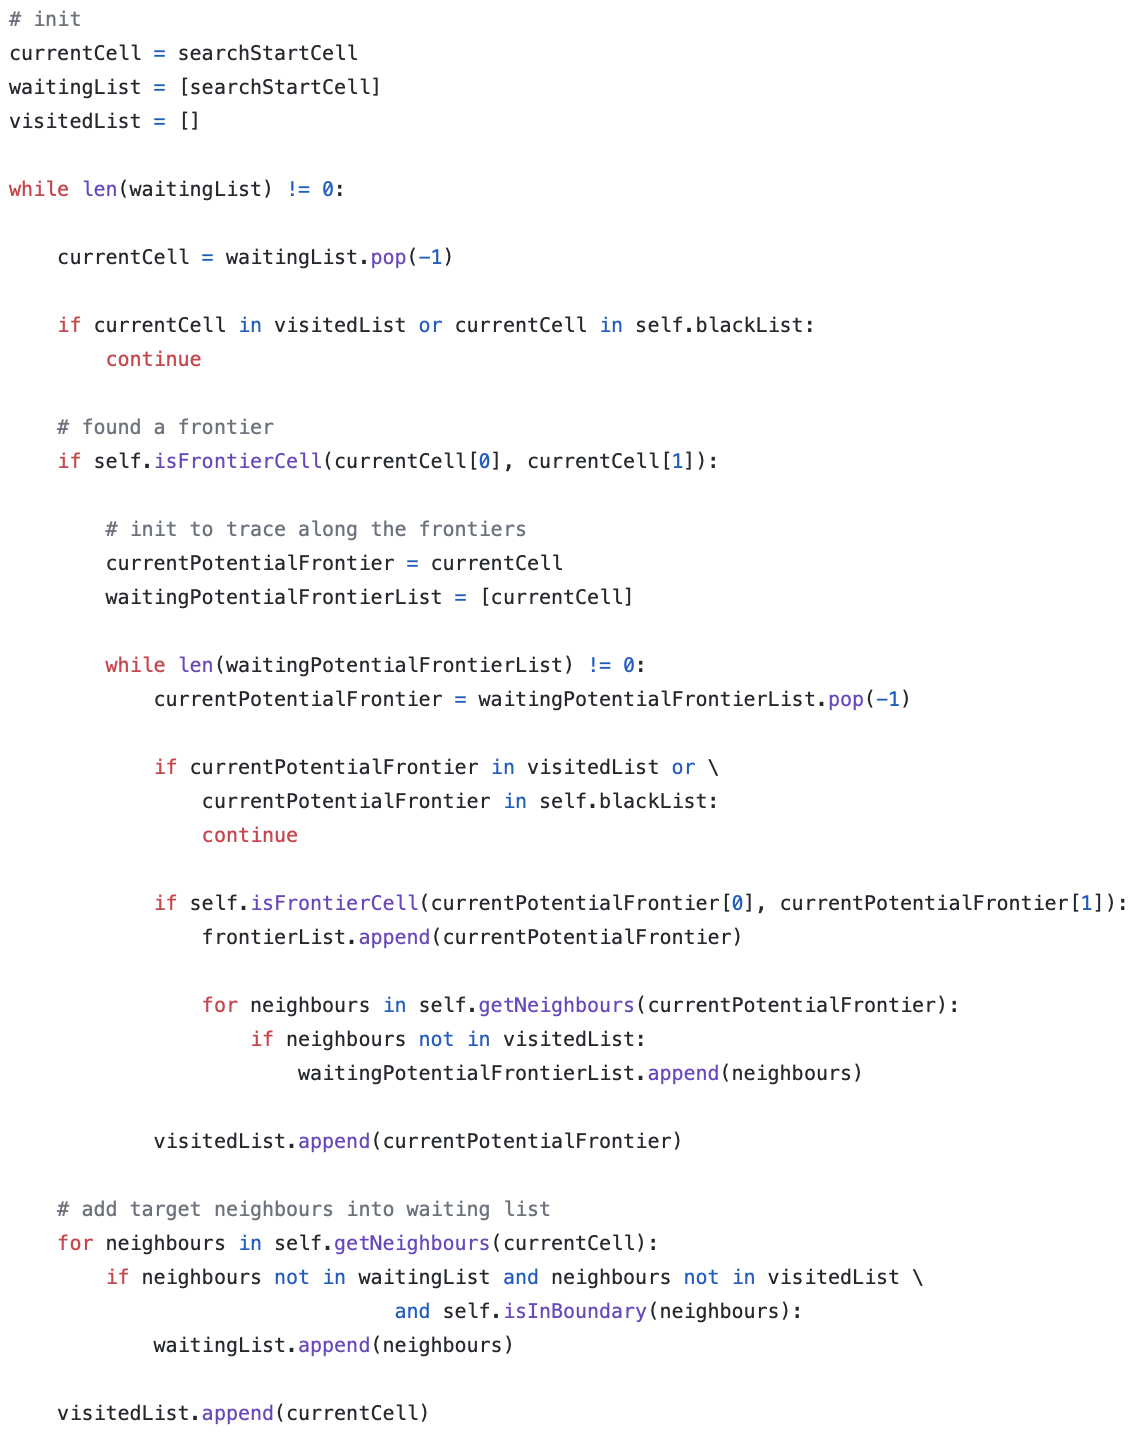
\includegraphics[scale=0.5]{graphs/part2/2-3/WaveFrontDetection.png}
\caption{Wave Front Detection}
\label{fig:waveFrontDetection}
\end{figure}

\begin{figure}[ht]
\centering
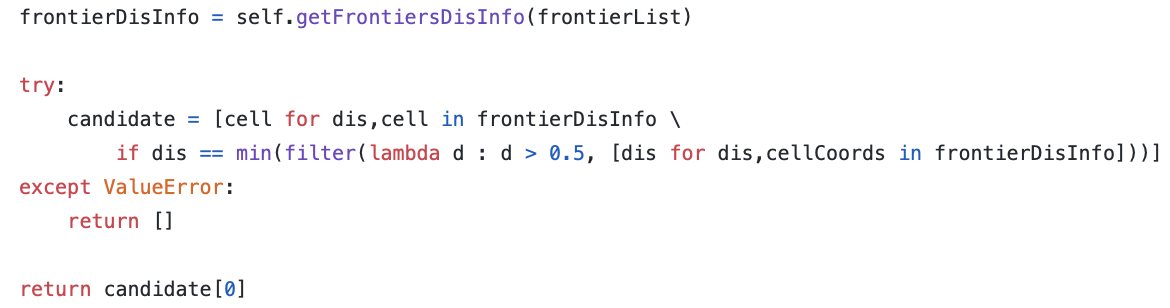
\includegraphics[scale=0.5]{graphs/part2/2-3/closest.png}
\caption{Closest Heuristic}
\label{fig:closestHeuristic}
\end{figure}

Specifically, we implement the wave front detection using two nested breadth first search referencing from the suggested paper 'Frontier Based Exploration for Autonomous Robot' \cite{WFD}. The outer one goes through the normal cells starting from the current robot position and checks if the current cell is a frontier or not. If the current cell is a frontier and is not visited yet, it enters the inner loop and adds the cell into the frontier list if the cell. At the end of both loops, the valid unvisited neighbours (the 'valid' means it is not out of boundary) of the current (frontier) cell will be pushed into the waiting list. It is notable that the neighbours of a frontier cell are much more likely to be frontiers.To get the closest frontier from the current robot position, we first calculate the distance and store the information into a list \textit{fronterDisInfo} along with the cell coordinate, and then use the list comprehensions. Due to limitation of the \textit{min()}, we add an exception to handle the error occurred when there is no cell in the list after removing the frontier cells that are too close to the robot. 

As a result, the new algorithm takes around 30 minutes to explores the map with 78.24 \% coverage. 

\pagebreak
% -------------------------------------------------------------------------------------------
\section{Integration of Our Planner and Exploration System}

See Fig.\ref{fig:result3} for the result. The coverage is  78.31\%.

\begin{figure}[H]
\centering  
\subfigure[STDR GUI]{
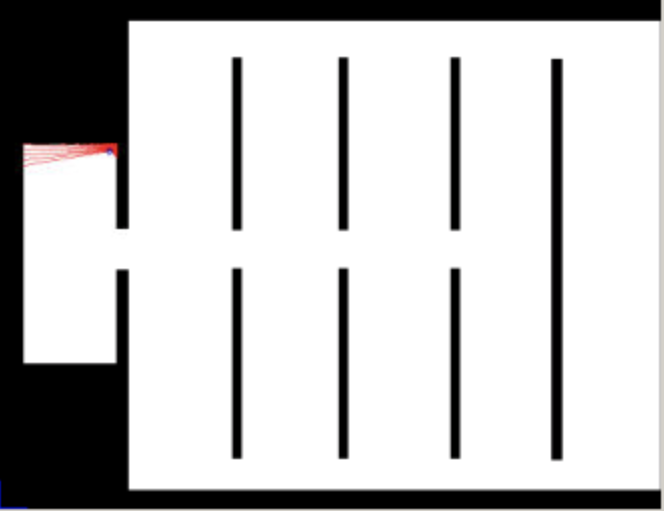
\includegraphics[width=0.45\textwidth]{graphs/part3/GUI.png}}
\subfigure[Planner Occupancy Grid]{
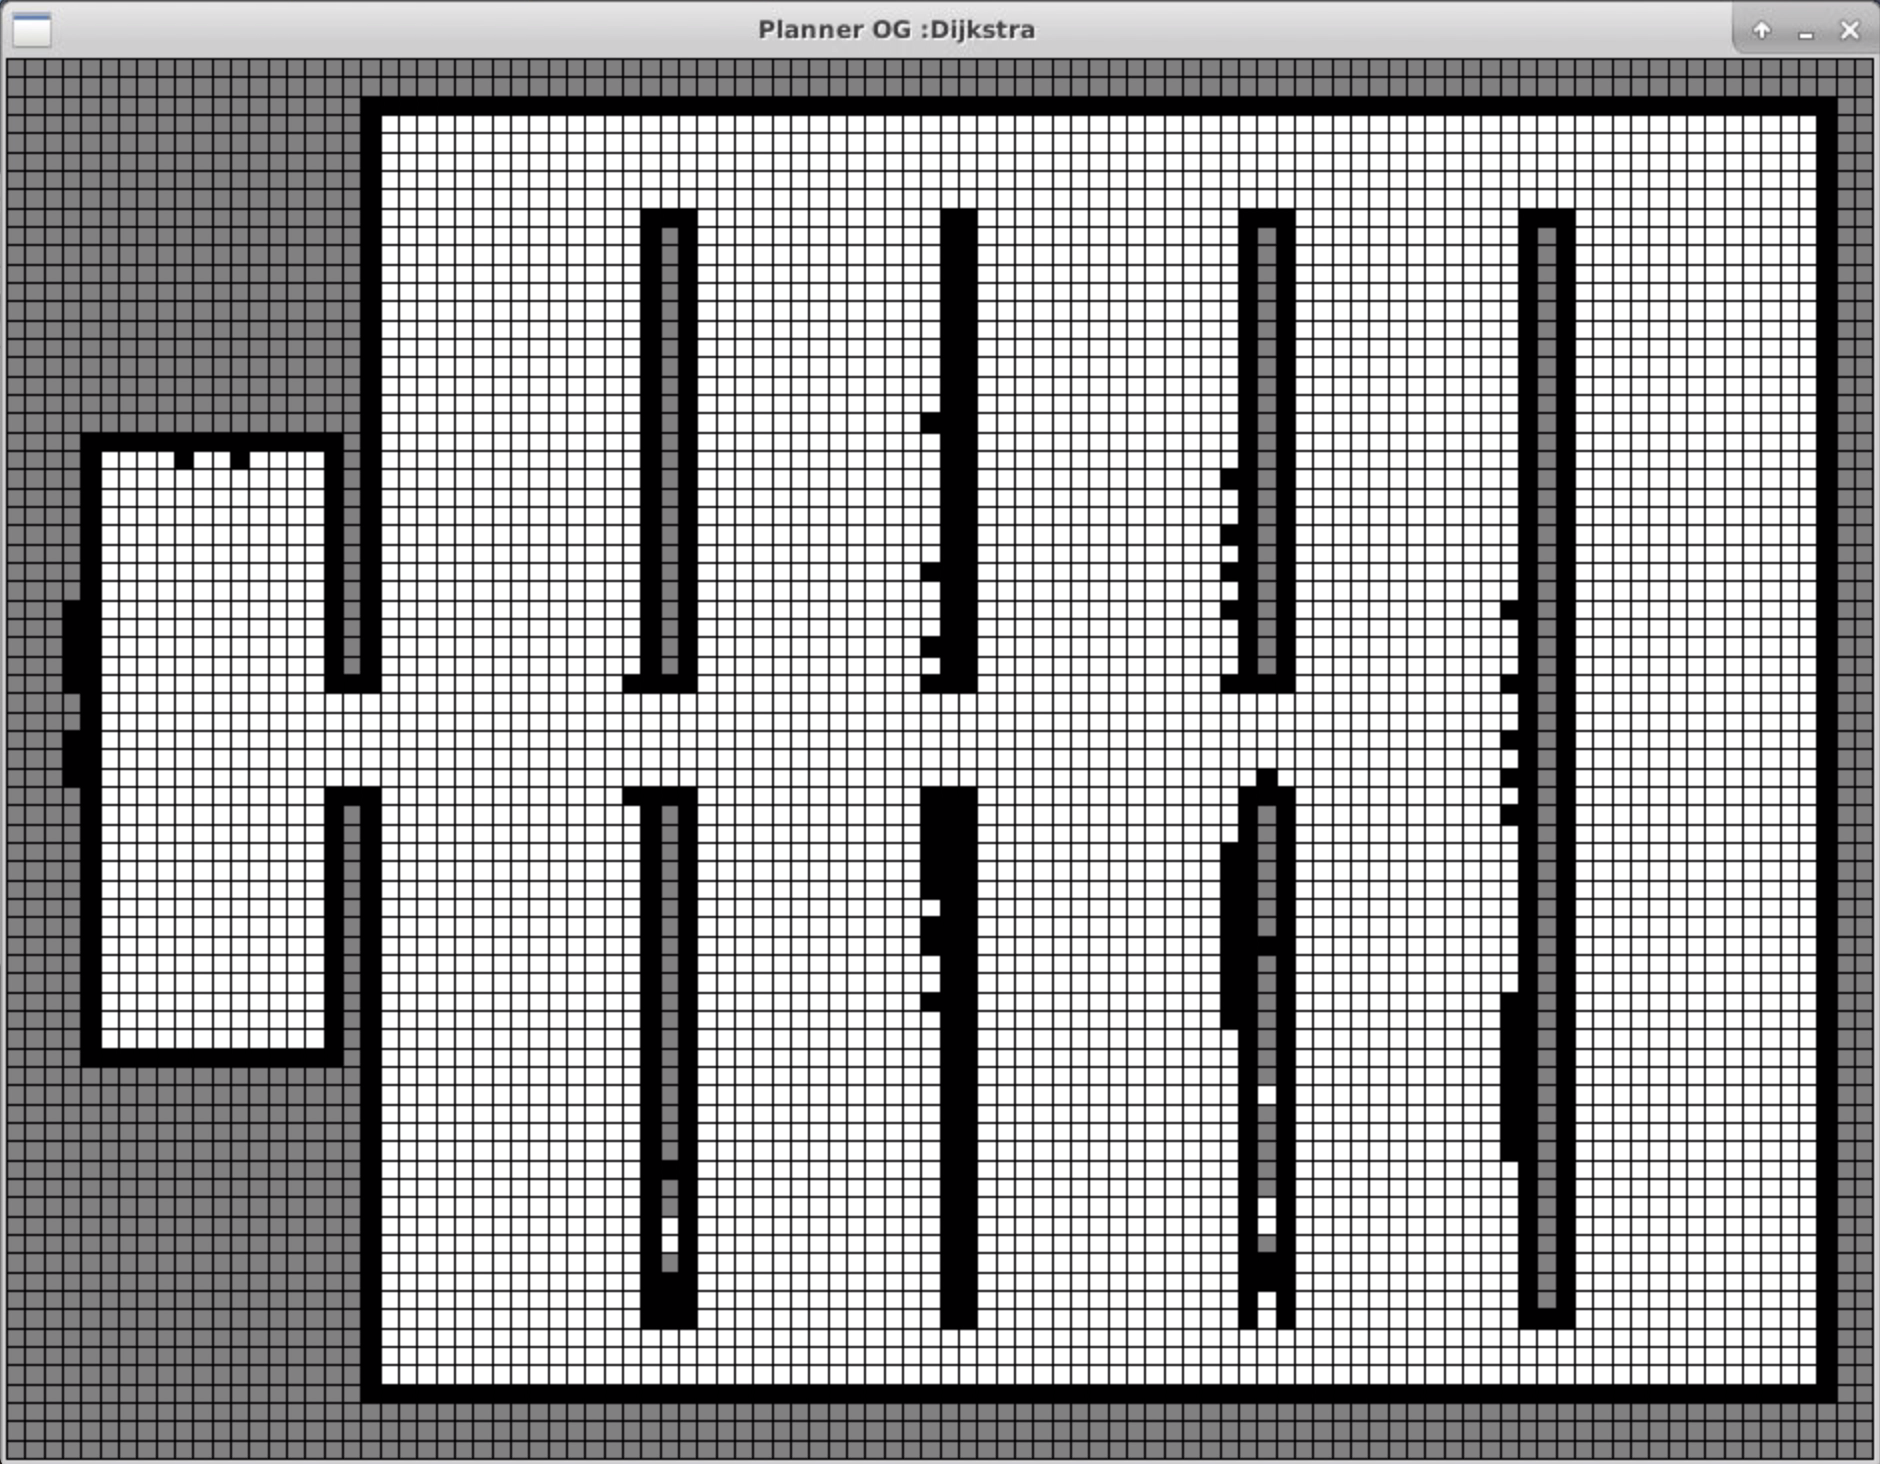
\includegraphics[width=0.45\textwidth]{graphs/part3/plannerOG.png}}
\subfigure[Planner Search Grid]{
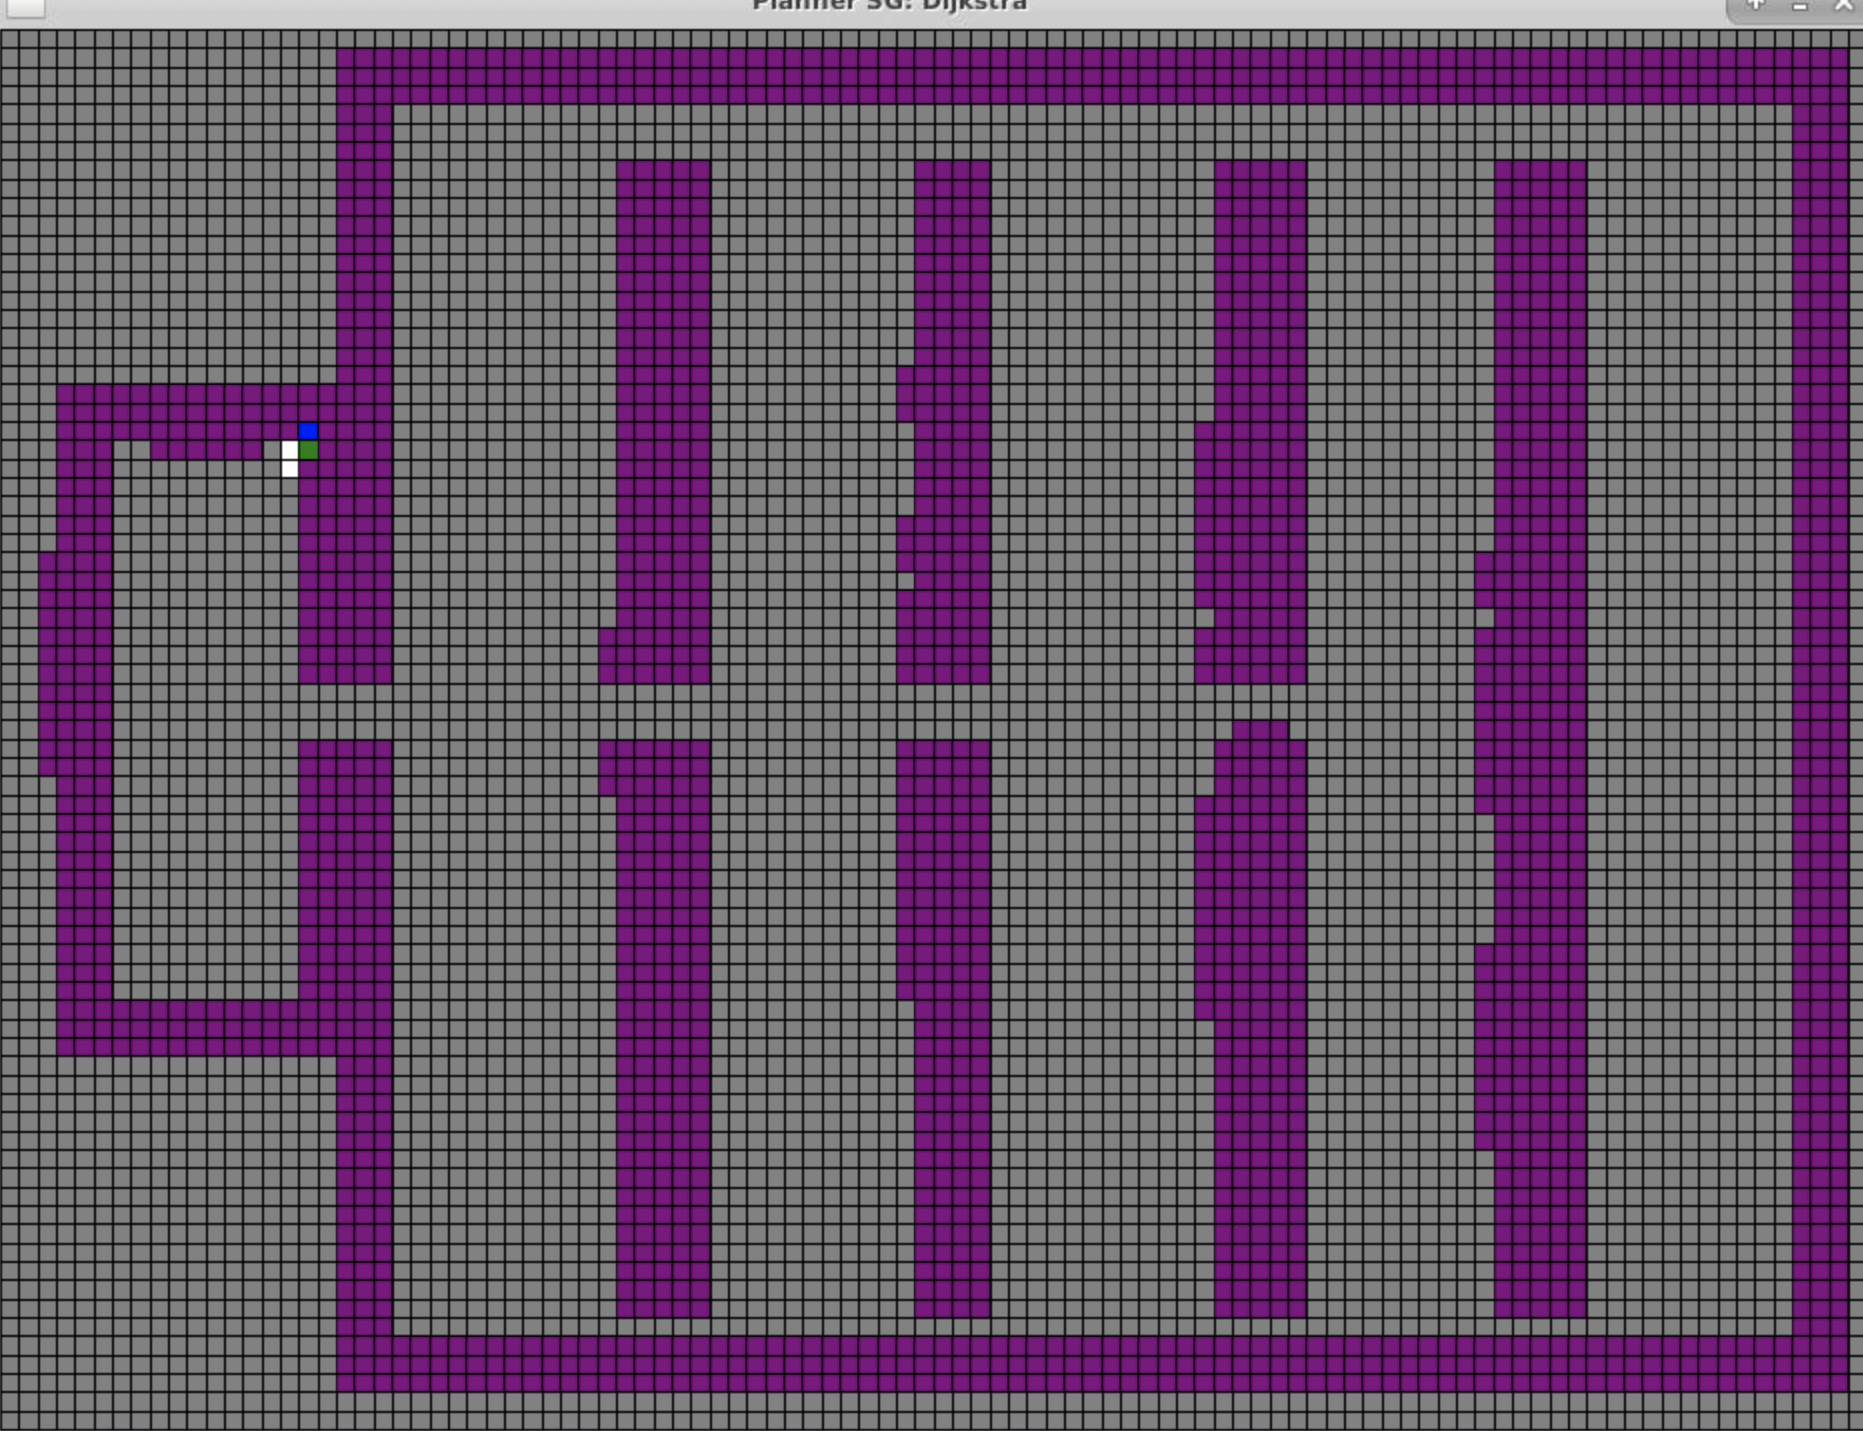
\includegraphics[width=0.45\textwidth]{graphs/part3/plannerSG.png}}
\subfigure[Mapper Node Occupancy Grid]{
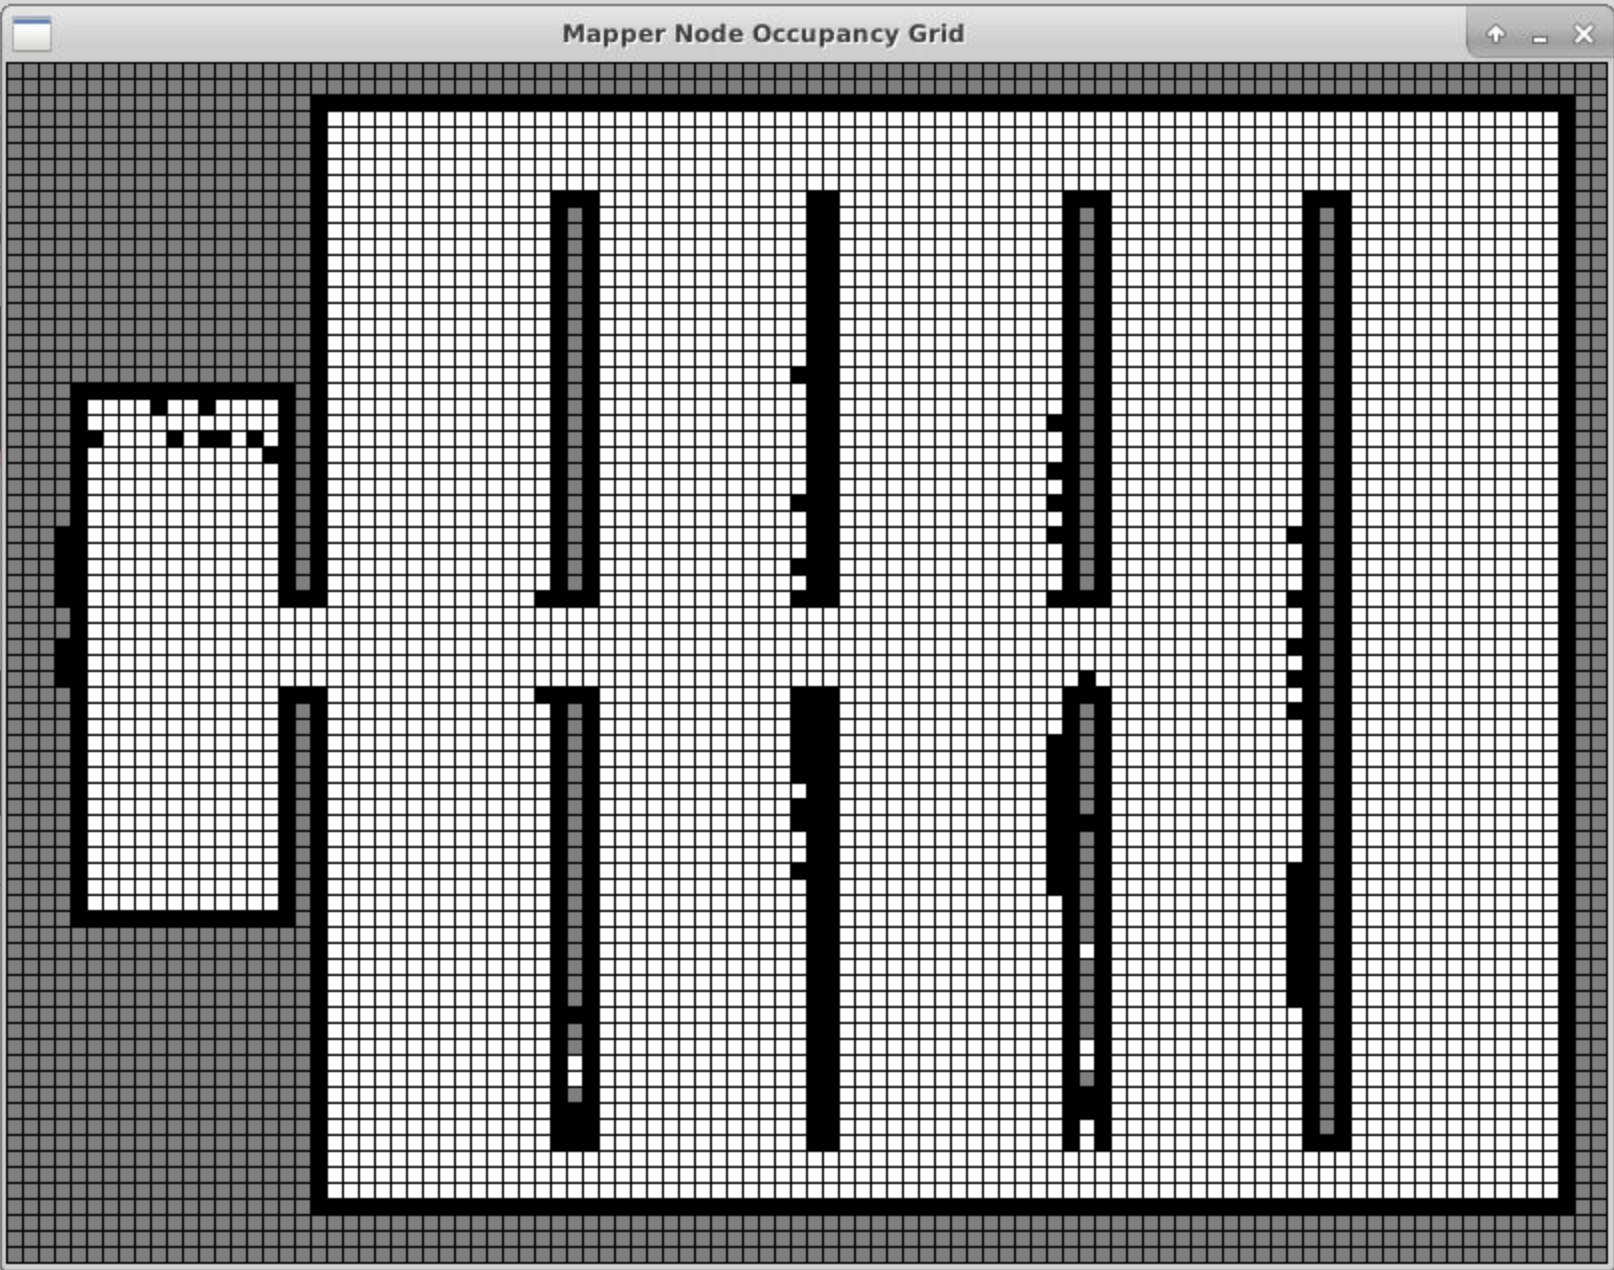
\includegraphics[width=0.45\textwidth]{graphs/part3/mapperNodeOG.png}}
\caption{Result on the second launch script}
\label{fig:result3}
\end{figure}

\pagebreak
% -------------------------------------------------------------------------------------------
\section{Information-Theoretic Path Planning}
% ----------------
\subsection {Definition}
In terms of path planning, the information theoritic approach picks the next waypoint which can reduce the uncertainty of map the most. One approach is using entropy, which based on the thermodynamic concept of irregularity, to assess the uncertainty. And to decide where to go, mutual entropy is used. In detail, it first pick a location and predict the observation. If it saw the observation, then update the map and check the effect on the map entropy. In our model where cells are either empty (0), unknown (0.5) and blocked (1), the entropy of a single cell is:

\begin{align}
H(C) &= - \sum p(c=c)ln(c=c) \\
         &= -(1-p(c))ln(1-p(c)) - p(c)ln\,p(c) \\
\end{align}

And the mutual information is given by:
\begin{align}
I(x) = H(C) - H(C|x) 
\end{align}

Where H(C|x) is the expected entropy  such that 
\begin{align}
H(C|x)= \sum_{C}p_{C_{k}} (M) H(C|x, z(M))
\end{align}
Where x, z is the destination and observation
% ----------------
\subsection{Our Modification}
In our model, we simply use the following equation to compute the entropy of the map once every 5 seconds of simulation time (the code is shown in Fig.\ref{fig:calculateEntropy}).
\begin{equation}
p_{c}(M) = |C_{U}|ln(2)
\end{equation}

\begin{figure}[H]
\centering  
\subfigure[]{
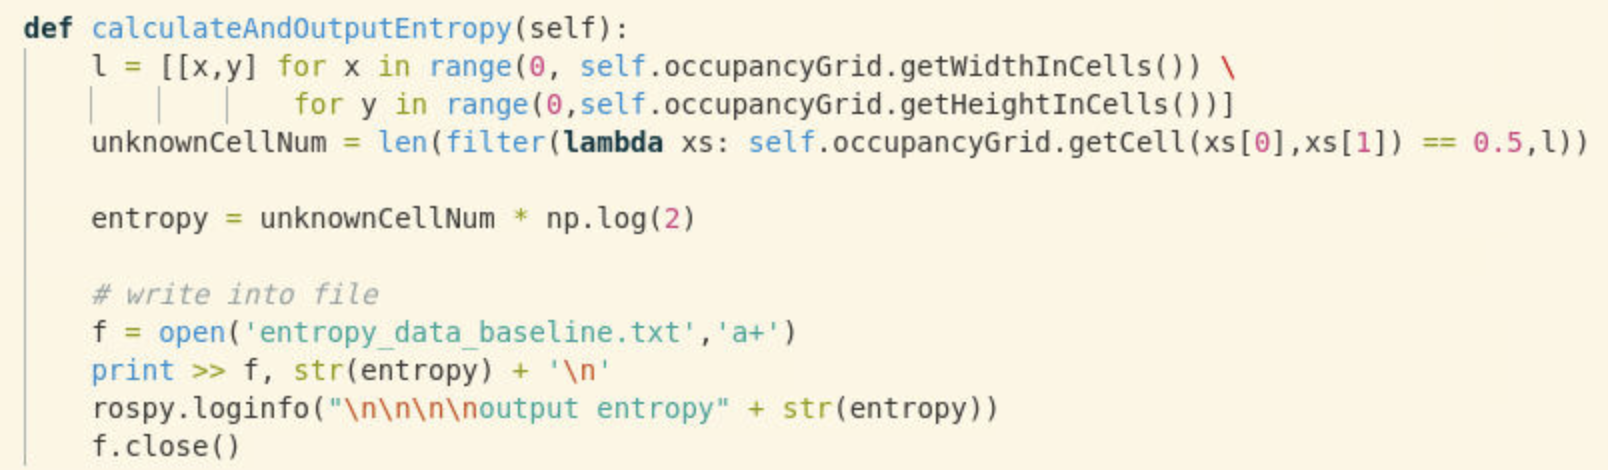
\includegraphics[width=0.8\textwidth]{graphs/part4/4-2/1.png}}
\subfigure[]{
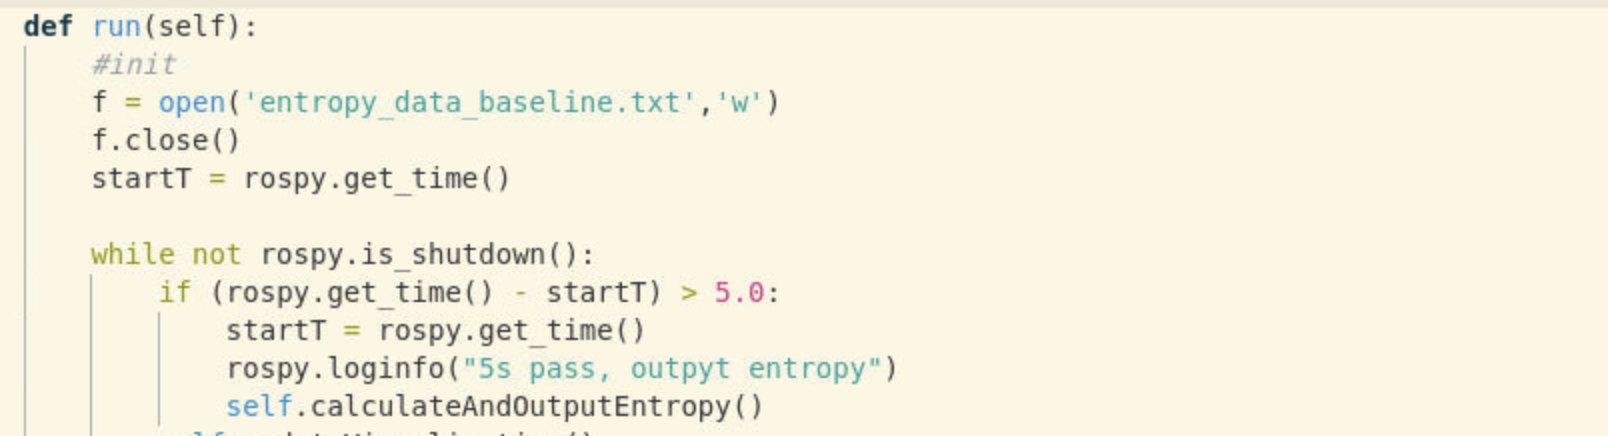
\includegraphics[width=0.8\textwidth]{graphs/part4/4-2/2.png}}
\caption{Our Implementation}
\label{fig:calculateEntropy}
\end{figure}

% ----------------
\subsection{Performance Evaluation}
As shown in the graph (Fig.\ref{fig:entropyGraph}), the two approach give similar performance with after 300 time steps (i.e, 1500 seconds after starting) the baseline algorithm outweigh the others, though theoretically the wave front detection should have a better performance. The total time to explore the map used by the two approaches (mentioned in the previous sections) also support that. We think the reason may be due to that the way we implement the detection approach makes the searching frontiers phase take too much time. Besides this main reason, during the exploration, we found that in most cases the robot will choose to go out of the initial room first instead of exploring the room corner. Then the robot has to re-enter the room later. In addition, we found that, since it will always pick the closest frontier, and whenever the robot reaches the destination, the search frontier phase will be called. As a result, even if the robot has not moved forward for a significant distance, the search algorithm has been called multiple times,  each time with a non-negligible cost. Based on our situation, we will suggest that the baseline algorithm is more effective.

\begin{figure}[ht]
\centering
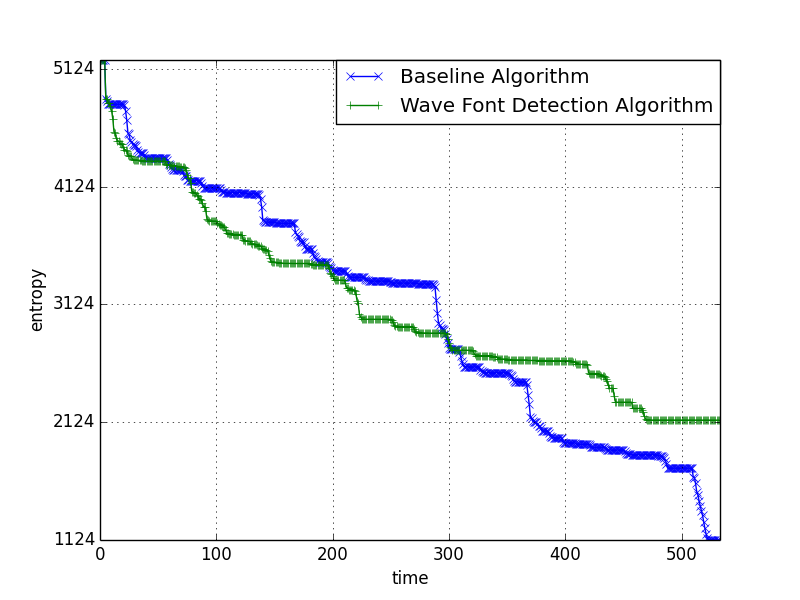
\includegraphics[scale=0.5]{graphs/part4/4-3/entropy.png}
\caption{}
\label{fig:entropyGraph}
\end{figure}

\pagebreak
% -------------------------------------------------------------------------------------------

\bibliographystyle{unsrt}  
\begin{thebibliography}{1}


 \bibitem{WFD}
 Anirudh Topiwala; Pranav Inani; Abhishek Kathpal
\newblock (2018)
\newblock Frontier Based Exploration for Autonomous Robot
\newblock {\em<https://arxiv.org/abs/1806.03581>}.

 \bibitem{2}
Brian Yamauchi
\newblock (1997)
\newblock  A Frontier-Based Approach for Autonomous Exploration
\newblock {\em<https://www.semanticscholar.org/paper/A-frontier-based-approach-for-autonomous-Yamauchi/a1875055e9c526cbdc7abb161959d76d14b58266>}.

 \bibitem{InfoTheoretic}
Callum Rhodes; Cunjia Liu; Wen-Hua Chen
\newblock (2019)
\newblock An Information Theoretic Approach to Path Planning for Frontier Exploration
\newblock {\em<https://www.researchgate.net/publication/331929185\_An\_Information\_Theoretic\_Approach\_to\_Path\_Planning\_for\_Frontier\_Exploration>}.

 \bibitem{3}
Steven M. LaValle
\newblock (2006)
\newblock Planning Algorithm
\newblock {\em<http://planning.cs.uiuc.edu>}.

 \bibitem{4}
Matan Keidar; Gal A. Kaminka
\newblock Efficient Frontier Detection for Robot Exploration
\newblock Volume: 33 issue: 2
\newblock page(s):215-236
\newblock First published online: October 22, 2013
\newblock Issue published: February 1, 2014

 \bibitem{5}
Robert M. Gray
\newblock (2013)
\newblock Entropy and Information Theory
\newblock {\em<https://ee.stanford.edu/\~gray/it.pdf>}.



\end{thebibliography}


% -----------------------------------------------------------------------------------------
\end{document}